% Options for packages loaded elsewhere
\PassOptionsToPackage{unicode}{hyperref}
\PassOptionsToPackage{hyphens}{url}
\PassOptionsToPackage{dvipsnames,svgnames,x11names}{xcolor}
%
\documentclass[
  10pt,
  a4paper,
]{article}
\usepackage{amsmath,amssymb}
\usepackage{iftex}
\ifPDFTeX
  \usepackage[T1]{fontenc}
  \usepackage[utf8]{inputenc}
  \usepackage{textcomp} % provide euro and other symbols
\else % if luatex or xetex
  \usepackage{unicode-math} % this also loads fontspec
  \defaultfontfeatures{Scale=MatchLowercase}
  \defaultfontfeatures[\rmfamily]{Ligatures=TeX,Scale=1}
\fi
\usepackage{lmodern}
\ifPDFTeX\else
  % xetex/luatex font selection
  \setmainfont[]{Latin Modern Roman}
  \setsansfont[]{Latin Modern Sans}
  \setmonofont[]{Latin Modern Mono}
\fi
% Use upquote if available, for straight quotes in verbatim environments
\IfFileExists{upquote.sty}{\usepackage{upquote}}{}
\IfFileExists{microtype.sty}{% use microtype if available
  \usepackage[]{microtype}
  \UseMicrotypeSet[protrusion]{basicmath} % disable protrusion for tt fonts
}{}
\makeatletter
\@ifundefined{KOMAClassName}{% if non-KOMA class
  \IfFileExists{parskip.sty}{%
    \usepackage{parskip}
  }{% else
    \setlength{\parindent}{0pt}
    \setlength{\parskip}{6pt plus 2pt minus 1pt}}
}{% if KOMA class
  \KOMAoptions{parskip=half}}
\makeatother
\usepackage{xcolor}
\usepackage[margin=23mm]{geometry}
\usepackage{longtable,booktabs,array}
\usepackage{calc} % for calculating minipage widths
% Correct order of tables after \paragraph or \subparagraph
\usepackage{etoolbox}
\makeatletter
\patchcmd\longtable{\par}{\if@noskipsec\mbox{}\fi\par}{}{}
\makeatother
% Allow footnotes in longtable head/foot
\IfFileExists{footnotehyper.sty}{\usepackage{footnotehyper}}{\usepackage{footnote}}
\makesavenoteenv{longtable}
\usepackage{graphicx}
\makeatletter
\def\maxwidth{\ifdim\Gin@nat@width>\linewidth\linewidth\else\Gin@nat@width\fi}
\def\maxheight{\ifdim\Gin@nat@height>\textheight\textheight\else\Gin@nat@height\fi}
\makeatother
% Scale images if necessary, so that they will not overflow the page
% margins by default, and it is still possible to overwrite the defaults
% using explicit options in \includegraphics[width, height, ...]{}
\setkeys{Gin}{width=\maxwidth,height=\maxheight,keepaspectratio}
% Set default figure placement to htbp
\makeatletter
\def\fps@figure{htbp}
\makeatother
\setlength{\emergencystretch}{3em} % prevent overfull lines
\providecommand{\tightlist}{%
  \setlength{\itemsep}{0pt}\setlength{\parskip}{0pt}}
\setcounter{secnumdepth}{5}
% definitions for citeproc citations
\NewDocumentCommand\citeproctext{}{}
\NewDocumentCommand\citeproc{mm}{%
  \begingroup\def\citeproctext{#2}\cite{#1}\endgroup}
\makeatletter
 % allow citations to break across lines
 \let\@cite@ofmt\@firstofone
 % avoid brackets around text for \cite:
 \def\@biblabel#1{}
 \def\@cite#1#2{{#1\if@tempswa , #2\fi}}
\makeatother
\newlength{\cslhangindent}
\setlength{\cslhangindent}{1.5em}
\newlength{\csllabelwidth}
\setlength{\csllabelwidth}{3em}
\newenvironment{CSLReferences}[2] % #1 hanging-indent, #2 entry-spacing
 {\begin{list}{}{%
  \setlength{\itemindent}{0pt}
  \setlength{\leftmargin}{0pt}
  \setlength{\parsep}{0pt}
  % turn on hanging indent if param 1 is 1
  \ifodd #1
   \setlength{\leftmargin}{\cslhangindent}
   \setlength{\itemindent}{-1\cslhangindent}
  \fi
  % set entry spacing
  \setlength{\itemsep}{#2\baselineskip}}}
 {\end{list}}
\usepackage{calc}
\newcommand{\CSLBlock}[1]{\hfill\break\parbox[t]{\linewidth}{\strut\ignorespaces#1\strut}}
\newcommand{\CSLLeftMargin}[1]{\parbox[t]{\csllabelwidth}{\strut#1\strut}}
\newcommand{\CSLRightInline}[1]{\parbox[t]{\linewidth - \csllabelwidth}{\strut#1\strut}}
\newcommand{\CSLIndent}[1]{\hspace{\cslhangindent}#1}
\ifLuaTeX
\usepackage[bidi=basic]{babel}
\else
\usepackage[bidi=default]{babel}
\fi
\babelprovide[main,import]{british}
\ifPDFTeX
\else
\babelfont{rm}[]{Latin Modern Roman}
\fi
% get rid of language-specific shorthands (see #6817):
\let\LanguageShortHands\languageshorthands
\def\languageshorthands#1{}
\usepackage{caption}
\usepackage{fancyhdr}
\usepackage{titlesec}
\usepackage{needspace}
\usepackage{float}
\definecolor{papernavy}{HTML}{172E41}
\definecolor{paperteal}{HTML}{006F73}
\titleformat{\section}{\normalfont\Large\bfseries\color{papernavy}}{\thesection}{0.7em}{}
\titleformat{\subsection}{\normalfont\large\bfseries\color{papernavy}}{\thesubsection}{0.65em}{}
\captionsetup{font=small,labelfont=bf}
\pagestyle{fancy}
\fancyhf{}
\fancyhead[L]{\footnotesize\sffamily Aave Liquidation Stress}
\fancyhead[R]{\footnotesize Research revision}
\fancyfoot[R]{\small\thepage}
\renewcommand{\headrulewidth}{0.3pt}
\setlength{\headheight}{15pt}
\setlength{\parskip}{5pt}
\linespread{1.11}
\emergencystretch=2em
\ifLuaTeX
  \usepackage{selnolig}  % disable illegal ligatures
\fi
\usepackage{bookmark}
\IfFileExists{xurl.sty}{\usepackage{xurl}}{} % add URL line breaks if available
\urlstyle{same}
\hypersetup{
  pdftitle={Early Warning of Aave Liquidation Stress under Delayed and Incomplete Network Data},
  pdflang={en-GB},
  pdfkeywords={decentralised finance, liquidation stress, temporal
graphs, calibration, transfer learning, data provenance},
  colorlinks=true,
  linkcolor={teal},
  filecolor={Maroon},
  citecolor={Blue},
  urlcolor={teal},
  pdfcreator={LaTeX via pandoc}}

\title{Early Warning of Aave Liquidation Stress under Delayed and
Incomplete Network Data}
\usepackage{etoolbox}
\makeatletter
\providecommand{\subtitle}[1]{% add subtitle to \maketitle
  \apptocmd{\@title}{\par {\large #1 \par}}{}{}
}
\makeatother
\subtitle{Chronological forecasting, reliability-aware fusion and
conditional cross-protocol transfer}
\author{}
\date{Revised research manuscript - 17 November 2026}

\begin{document}
\maketitle
\begin{abstract}
Network measurements can inform liquidation monitoring only if they add
predictive value to timely local information and remain useful when
observations deteriorate. We evaluate daily tail-volume warnings for the
Ethereum Aave V2 and V3 series using event-level liquidation records,
timestamped reserve and oracle inputs, and weekly global
protocol-exposure graphs. Three chronological test folds contain 1,022
forecasts and 110 positive outcomes. Recomputed average precision is
0.1954 for a calibrated temporal graph ensemble, 0.2479 for the matched
market-augmented GRU and 0.3127 for prior-day liquidation. The
graph-minus-GRU AP difference is -0.0525, with a paired 14-day block
interval of {[}-0.1488, 0.0161{]}. Across 100 edge-removal masks per
rate, ranking and probability accuracy respond differently. A previously
unscored later Aave window contains 744 forecasts and 40 positives: a
learned reliability gate obtains AP 0.3230 and Brier 0.04644, versus
0.3242 and 0.04626 for the GRU. Newly trained common-schema models are
transferred with frozen source weights to published Compound histories.
Ranking transfer is weak, but inference is conditional on an
outlier-filtered daily dataset with five missing dates, including 5
August 2024. Independent contract reconciliation and a representative
historical Health Factor baseline remain unresolved. The evidence
documents conditional forecasting performance and failure modes, rather
than a demonstrated network or fusion advantage.
\end{abstract}

\section{Introduction}\label{introduction}

Public blockchain records expose events that are difficult to observe in
conventional credit markets. That visibility does not make tomorrow's
aggregate liquidation volume straightforward to predict. Position
eligibility depends on collateral, debt, prices and protocol rules;
realised liquidation additionally depends on borrower adjustments,
execution incentives and available liquidity. Empirical work documents
liquidation incentives and execution frictions (Qin et al. 2021; Schuler
2026). An early-warning study must therefore define its outcome
precisely. Here it is unusually large \emph{realised, source-reported
USD liquidation volume}, not the probability that an individual borrower
becomes insolvent.

The potential contribution of network information is conditional. A
token-mediated link might contain information beyond recent
liquidations, reserve conditions and market prices. It might instead
reflect common price movements, protocol scale or retrospective data
construction. DeXposure supplies historical measurements of global
inter-protocol exposure (Wu et al. 2025). Matching them to Ethereum Aave
outcomes permits a predictive comparison under an explicit lag
assumption. It does not identify causal transmission or establish that a
published historical graph was obtainable on each forecast date.

We ask whether a temporal graph improves ranking or probability loss
over the same timed local/market inputs; whether disagreement-based
fusion protects forecasts when network observations deteriorate; and
whether common-schema Aave models transfer to Compound. The last
question is conditional because the available Compound dataset has
material provenance and calendar limitations. A fourth question is
specified but remains untested: whether networks add information after a
representative historical borrower Health Factor panel is included.

The contribution is an auditable benchmark and a set of negative or
qualified findings. We distinguish score recomputation from model
refitting, corruption draws from independent training repetitions,
chronological novelty from independent source validation, and actual
weight transfer from a separately fitted external benchmark. A later
Aave holdout extends evaluation beyond the previously inspected
calendar. Every reported result comes from a saved ledger; unfinished
analyses are listed explicitly.

\section{Related research}\label{related-research}

\subsection{Liquidation mechanisms and realised
distress}\label{liquidation-mechanisms-and-realised-distress}

Qin et al. (2021) compare liquidation mechanisms and examine incentives
and borrower losses. Lehar and Parlour (2022) study interactions between
liquidation and decentralised trading. These mechanisms motivate
monitoring aggregate pressure but require more evidence than a
forecasting coefficient to establish contagion. Chiu and Danisman (2026)
document leverage and concentrated liquidation waves in Aave V3. Schuler
(2026) distinguish undercollateralisation from subsequent execution in
Aave V2. Our daily outcome aggregates such processes rather than
estimating account-level transition probabilities.

The cross-version study of Iftikhar, Wei, and Cartlidge (2025) uses
daily Aave and Compound data for panel regression. Its repository
supplies our external series. Regression and tail-warning studies have
different data requirements: removing extreme observations may be a
regression robustness choice, while removing a crisis day directly
compromises a stress benchmark. We therefore inspect the full calendar
and retain the fact of exclusion in every transfer interpretation. A
named liquidation column is not treated as contract-level validation.

\subsection{Network learning and
transfer}\label{network-learning-and-transfer}

DeXposure reconstructs global token-mediated relationships and
benchmarks clustering, exposure dynamics and link prediction (Wu et al.
2025). DeXposure-FM extends this setting to flow and graph forecasting
(Shu et al. 2026). Their outcomes differ from realised next-day
liquidation warnings. We use a weighted inductive neighbour encoder
inspired by GraphSAGE (Hamilton, Ying, and Leskovec 2017) followed by a
GRU (Cho et al. 2014). The non-graph GRU is the central matched
comparator. Predicting topology well does not guarantee incremental
liquidation information conditional on local histories and prices.

Transfer is more demanding than evaluating models on two datasets.
Source weights, feature transforms, stopping rules and calibration must
remain fixed during target prediction. Feature meanings and target
definitions must also be aligned. We train new shared-schema variants
and distinguish them from the original reserve-augmented models. The
experiment tests that common representation under documented
assumptions; it does not establish portability of every original
predictor or checkpoint.

\subsection{Calibration, disagreement and
decisions}\label{calibration-disagreement-and-decisions}

Average precision (AP) measures rare-event ranking, while Brier score
and log loss measure probability quality (Saito and Rehmsmeier 2015;
Gneiting and Raftery 2007). These objectives can disagree. Calibration
can improve probability loss without creating new information (Guo et
al. 2017). Deep ensembles measure variation across fitted members
(Lakshminarayanan, Pritzel, and Blundell 2017), but their spread is not
a complete uncertainty measure. All members can share a misspecification
or use the same obsolete graph. Distribution-shift evidence motivates
evaluation beyond the original calendar (Ovadia et al. 2019).

Selective classification studies retained coverage and error (Geifman
and El-Yaniv 2017). A monitoring interface must additionally count
manual review and missed episode onsets. We distinguish a review queue,
which defers a case, from a probability mixture, which changes its
forecast. Neither is considered useful merely because it lowers a
conditional error or marginally improves one ranking score.

\section{Data, provenance and timing}\label{data-provenance-and-timing}

\subsection{Primary Aave cohort}\label{primary-aave-cohort}

The primary calendar is 1 March 2023-24 August 2025. Each forecast
concerns one archive-labelled Ethereum Aave version at UTC midnight. The
pinned Chaffard release supplies liquidation events, paired hourly
aggregates, reserve histories and Chainlink oracle updates (Chaffard
2026). Reserve inputs cover DAI, USDC, USDT and WETH. Event IDs and
transaction-hash/log-index pairs are unique. Event sums and counts
reconcile to the publisher's hourly tables. This is internal
consistency, not independent reconstruction of every contract log or USD
valuation.

The graph is pinned to DeXposure commit
\texttt{79071f26ddb3cf59adb433fb277bc820732bf863}, with 283 weekly
snapshots through 18 August 2025. AAVE V2 is node 111 and AAVE V3 node
1599. Global protocol coverage is broader than Ethereum outcomes.
Self-links, unmapped entities and nonpositive/nonfinite weights are
excluded, repeated pairs are summed and up to 16 neighbours per
direction are retained by weight. A snapshot is eligible only when it is
at least seven days old.

\Needspace{10\baselineskip}
\begin{longtable}[]{@{}
  >{\raggedright\arraybackslash}p{(\columnwidth - 4\tabcolsep) * \real{0.3333}}
  >{\raggedright\arraybackslash}p{(\columnwidth - 4\tabcolsep) * \real{0.3333}}
  >{\raggedright\arraybackslash}p{(\columnwidth - 4\tabcolsep) * \real{0.3333}}@{}}
\toprule\noalign{}
\begin{minipage}[b]{\linewidth}\raggedright
Input
\end{minipage} & \begin{minipage}[b]{\linewidth}\raggedright
Forecast-time restriction
\end{minipage} & \begin{minipage}[b]{\linewidth}\raggedright
Interpretation
\end{minipage} \\
\midrule\noalign{}
\endhead
\bottomrule\noalign{}
\endlastfoot
Liquidation history & Events strictly before midnight & Prior realised
activity \\
Reserve state & Strictly prior observation; maximum age two days &
Selected reserve conditions \\
Oracle updates & Strictly prior actual update; maximum age three hours &
Returns, volatility, freshness \\
Exposure graph & Snapshot dated at least seven days earlier & Lagged
global context \\
Future events & Following 24 hours & Outcome only \\
\end{longtable}

These are retrospective releases. Source-event timestamp eligibility and
historical public availability are distinct. The seven-day graph lag is
an operational assumption, not a verified publication-time history.
Historically deployable performance would require revision-aware
acquisition logs. Mutable DefiLlama borrowing histories enter only the
original borrowing-scaled sensitivity, with their downloaded hashes
recorded separately.

\subsection{Run identity and
reproduction}\label{run-identity-and-reproduction}

The supplied main ledger and the existing GitHub ledger have identical
keys and labels, but 18,011 of 48,034 probabilities differ by more than
\(10^{-8}\). We use the supplied ledger consistently for the primary
results because its fusion and 100-mask extensions refer to that run;
columns from different runs are not mixed. All 47 model/scenario metric
rows recompute within \(8.4\times10^{-17}\) of the supplied tables. This
verifies score arithmetic and pairing, not unseen training-data
provenance.

A complete primary-model refit was executed from hash-matched raw
archives. Its temporal-graph AP rounds to 0.1949, versus 0.1954 in the
supplied ledger. The GRU, persistence and LightGBM headline scores agree
at reported precision. A neural stopping epoch differs in fold C, and
software environments differ. The subsequently available full aave.zip
upload contains all six original raw-file hashes. Its processed graph
values agree exactly with the reconstruction; panel differences are at
floating-point round-off scale. Both ledgers remain available;
byte-identical parquet or neural output is not asserted across Python
and numerical-library versions. These small headline differences leave
the interpretation unchanged.

\subsection{Compound source audit}\label{compound-source-audit}

The external CSV contains 1,456 rows from 1 January 2021 to 31 December
2024. Its date column is \texttt{Date}; the earlier feasibility manifest
incorrectly recorded a missing date field. The absent dates are 5 July,
1 August, 5 August, 25 November and 20 December 2024. The source paper
states that five outlier observations were removed (Iftikhar, Wei, and
Cartlidge 2025). We reindex the full calendar, preserve missing values
and exclude forecasts with an incomplete 14-step feature sequence.
Because each step includes a seven-day aggregate, validity can require
20 prior raw days. This leaves 196 scored days per Compound version in
April-December 2024.

Excluding the missing 5 August neighbourhood does not repair an
unfiltered crisis benchmark: it defines a sample omitting an important
stress episode. On 667 overlapping dates per Aave version, the external
Aave values and the pinned archive agree within USD 1. This establishes
numerical compatibility but does not prove independent ingestion or
validate Compound. Daily UTC alignment, exact deployment coverage and
contract-specific USD semantics remain assumptions for transfer.

\subsection{A previously unscored later
window}\label{a-previously-unscored-later-window}

A separate specification was recorded before scoring 25 August 2025-31
August 2026. The window contains 744 forecasts. Preparation of a longer
window first failed on four negative ETH/USD source observations on 15,
21 and 22 September 2026. Before generating later-window scores, we
capped evaluation at the last preceding complete calendar month.
September-November 2026 are quarantined. The amendment and final
specification hash accompany the results.

This uses the same Aave source: it is a new chronological test, not an
independent dataset or prospective deployment. No graph snapshots are
invented after the pinned release ends. Snapshot age grows from 7 to 378
days, deliberately creating a stale-feed regime. Performance here cannot
establish results with continuously refreshed networks.

\section{Methods}\label{methods}

\subsection{Outcome and chronological
separation}\label{outcome-and-chronological-separation}

Let \(V_{i,t}^{24}\) be source-reported liquidation USD for version
\(i\) in \([t,t+24\mathrm{h})\). The fold-specific target is
\[y_{i,t}^{(f)}=\mathbb{1}\{V_{i,t}^{24}>q_{i,f}\},\qquad q_{i,f}=Q_{0.95}\{V_{i,s}^{24}:s\in\mathcal T_f\}.\]
Thresholds use training outcomes only and differ by version. Tail
activity is relative to historical scale, not a universal insolvency
boundary. Thresholds and prevalence can change between folds.

Features include prior one-, three- and seven-day liquidation
sums/counts, borrowing and utilisation in four reserves, and a version
indicator. ETH/BTC channels contain one-/seven-day returns, daily
realised volatility, minimum hourly return and observation age. A tuning
interval selects neural stopping epochs; a subsequent calibration block
fits probability maps and warning cutoffs. Training, tuning and
calibration label windows end at least one day before the next
partition. Test outcome windows remain within their fold. Fourteen-day
input histories may precede a partition boundary because those
observations are already known; future outcomes never enter inputs.

\Needspace{10\baselineskip}
\begin{longtable}[]{@{}
  >{\raggedright\arraybackslash}p{(\columnwidth - 8\tabcolsep) * \real{0.2000}}
  >{\raggedright\arraybackslash}p{(\columnwidth - 8\tabcolsep) * \real{0.2000}}
  >{\raggedright\arraybackslash}p{(\columnwidth - 8\tabcolsep) * \real{0.2000}}
  >{\raggedright\arraybackslash}p{(\columnwidth - 8\tabcolsep) * \real{0.2000}}
  >{\raggedright\arraybackslash}p{(\columnwidth - 8\tabcolsep) * \real{0.2000}}@{}}
\caption{Original folds; exact inclusive dates and unrounded thresholds
are in run.json.}\tabularnewline
\toprule\noalign{}
\begin{minipage}[b]{\linewidth}\raggedright
Fold
\end{minipage} & \begin{minipage}[b]{\linewidth}\raggedright
Test origins
\end{minipage} & \begin{minipage}[b]{\linewidth}\raggedright
Train n
\end{minipage} & \begin{minipage}[b]{\linewidth}\raggedright
Test + / n
\end{minipage} & \begin{minipage}[b]{\linewidth}\raggedright
V2/V3 q95 (USD thousands)
\end{minipage} \\
\midrule\noalign{}
\endfirsthead
\toprule\noalign{}
\begin{minipage}[b]{\linewidth}\raggedright
Fold
\end{minipage} & \begin{minipage}[b]{\linewidth}\raggedright
Test origins
\end{minipage} & \begin{minipage}[b]{\linewidth}\raggedright
Train n
\end{minipage} & \begin{minipage}[b]{\linewidth}\raggedright
Test + / n
\end{minipage} & \begin{minipage}[b]{\linewidth}\raggedright
V2/V3 q95 (USD thousands)
\end{minipage} \\
\midrule\noalign{}
\endhead
\bottomrule\noalign{}
\endlastfoot
A & Apr-Jul 2024 & 610 & 33 / 244 & 493 / 106 \\
B & Aug-Dec 2024 & 852 & 24 / 306 & 617 / 416 \\
C & Jan-Aug 2025 & 1158 & 53 / 472 & 670 / 815 \\
\end{longtable}

\subsection{Models and fitting}\label{models-and-fitting}

Benchmarks include a smoothed training prior, a logistic persistence
predictor using prior-day liquidation, local/market logistic models and
shallow LightGBM with and without graph summaries (Ke et al. 2017). The
neural comparison uses the same 14-day history and a 24-unit GRU. Five
seeds (19, 43, 71, 101, 137) form each ensemble. Training uses
unweighted binary cross-entropy, AdamW at learning rate 0.001/weight
decay 0.001, batch size 64, gradient norm cap 2, at most 36 epochs and
tuning-loss patience seven.

The graph encoder transforms neighbour log size, log weight and an
availability flag through direction-specific multilayer maps. Normalised
exposure weights form incoming/outgoing means. These are joined with
local/market inputs and graph statistics: own size, age, total exposure,
retained degree, concentration and mean peer size. A linear layer, layer
normalisation and ReLU precede the GRU. Training-only scaling clips
standardised inputs to \([-12,12]\) and represents missing values with
zeros plus indicators. This tests a particular feature/model combination
rather than all graph architectures.

Static topology, one-step graph input, removal of market channels and
augmented training diagnose specific components. One-step models retain
engineered historical features and therefore are not information-free
about the past. No positive directed edge connects the two labelled Aave
version nodes in this extraction. The weighted cross-version interaction
consequently has no identifying variation and cannot support a causal
spillover estimate.

\subsection{Calibration, corruption and
review}\label{calibration-corruption-and-review}

The raw ensemble probability is the mean of five members; disagreement
is their variance. A positive-slope ridge Platt map is fitted on
calibration data and frozen. Probabilities are clipped to
\([10^{-6},1-10^{-6}]\) for log loss. An isotonic sensitivity remains in
the original ledgers.

Edge thinning removes retained links with probabilities 0.10, 0.30 or
0.50. Each mask is fixed within snapshot, version, direction and
neighbour slot. One fitted ensemble per fold is evaluated under 100
masks per rate; rates share nested draws. Empirical mask percentiles
describe corruption variability conditional on fixed weights, not
population confidence intervals or 100 training repetitions. Other
original scenarios add one oracle day, seven graph days, or both with
30\% thinning. Outcomes are held fixed; these are observation
disruptions, not market shocks.

An alert fires above the calibration-probability 90th percentile. A
separate review queue first defers cases above the
calibration-disagreement 90th percentile. Deferral does not count as
automated warning or successful analyst detection. Onsets are first
positive days after a nonpositive day or fold boundary. Lead time is
measured to cumulative target-volume threshold crossing, not necessarily
to the first liquidation.

\subsection{Reliability-aware fusion}\label{reliability-aware-fusion}

For calibrated graph/local forecasts \(p_G,p_L\) and graph disagreement
percentile \(r\), the fixed mixture uses \(w=1/2\) and the heuristic
uses \(w=(1-r)/2\): \[p_F=w p_G+(1-w)p_L.\] The learned gate is
\[w_\theta=\operatorname{sigmoid}(\theta_0+\theta_1r+\theta_2|p_G-p_L|+\theta_3p_G).\]
It minimises summed binary cross-entropy plus
\(\lambda\|\theta-\theta^{\mathrm{prior}}\|_2^2/2\), with prior
\((-1.5,-1,0,0)\). Original A predictions fit candidates and B selects
\(\lambda\in\{0.1,1,10,100\}\) by log loss; the selected value is 0.1.
For exploratory C evaluation, the gate is refitted on A/B. For the later
window, it is refitted on earlier A/B/C out-of-sample predictions. C was
already inspected when fusion was proposed, so C is not a fresh
discovery test.

The later base experts train through 29 April 2025, tune on 1 May-26
June and calibrate on 28 June-23 August. Later outcomes do not fit
experts, calibration, gate parameters or expiry rules. A specified
freshness comparator sets heuristic graph weight to zero when graph age
exceeds 28 days. This probes conservative fallback rather than learning
an optimal expiry. The later specification is retrospective and not
externally preregistered.

\subsection{Executed source-weight
transfer}\label{executed-source-weight-transfer}

Transfer variants replace reserve-specific channels with three shared
lagged-volume features,
\[x_{i,t}^{(k)}=\log\left(1+\frac{\sum_{j=1}^{k}V_{i,t-j}}{q_{i,\mathrm{train}}}\right),\quad k\in\{1,3,7\},\]
plus the same timed ETH/BTC inputs. The identity channel is constant
zero. Graph variants use the same neighbour encoder, with Compound nodes
114/2088. Aave alone fits source scaling, neural weights, stopping rules
and Platt calibration. Training covers 1 March-30 December 2023, tuning
1 January-13 February 2024, calibration 15 February-30 March and testing
April-December 2024.

Compound's 2023 q95 defines its target and unit normalisation. This use
of target history is explicit: the experiment is source-weight transfer
with target historical scaling, not zero information about the target.
No Compound label fits the transferred weights or calibration.
Separately trained Compound models provide supervised references under
the same chronology. They are distinct estimators, not fine-tuned source
models selected on target test scores. Paired comparisons use the same
valid target dates. The original reserve-augmented checkpoints are not
claimed to have been transferred.

\subsection{Scores and uncertainty}\label{scores-and-uncertainty}

We compute AP, Brier, log loss and AUROC from paired ledgers. A
moving-block bootstrap samples contiguous dates within each fold,
carrying both Aave versions and both models together (Künsch 1989). Main
contrasts retain 2,000 valid 14-day draws; original graph/GRU
comparisons also use seven-/28-day blocks. Percentile intervals
condition on fitted forecasts and observed regimes, omit refitting
uncertainty and are pointwise rather than simultaneous across all
contrasts. Further ablations and transfer contrasts are exploratory.
Failure to show a gain is not proof of equivalence.

\section{Results}\label{results}

\subsection{Original cohort and incremental graph
information}\label{original-cohort-and-incremental-graph-information}

The three original tests contain 1,022 cases and 110 positives.
Persistence has the strongest pooled AP among the listed original
predictors; the GRU has lower Brier loss than persistence. The temporal
graph does not establish incremental value over the GRU or graph-summary
tree comparison.

\Needspace{10\baselineskip}
\begin{longtable}[]{@{}llll@{}}
\caption{Primary clean scores recomputed from the supplied ledger; AP
higher and losses lower are preferable.}\tabularnewline
\toprule\noalign{}
Model & AP & Brier & Log loss \\
\midrule\noalign{}
\endfirsthead
\toprule\noalign{}
Model & AP & Brier & Log loss \\
\midrule\noalign{}
\endhead
\bottomrule\noalign{}
\endlastfoot
Training prior & 0.1150 & 0.0990 & 0.3645 \\
Prior-day liquidation & 0.3127 & 0.0918 & 0.3220 \\
Local logit & 0.2373 & 0.1038 & 0.3434 \\
LightGBM & 0.2574 & 0.0907 & 0.3264 \\
LightGBM + graph summaries & 0.2200 & 0.0926 & 0.3281 \\
Market + local GRU & 0.2479 & 0.0904 & 0.3129 \\
Static graph & 0.2324 & 0.0915 & 0.3176 \\
One-step graph & 0.2442 & 0.0906 & 0.3170 \\
Graph without market & 0.2226 & 0.0902 & 0.3100 \\
Graph raw & 0.1930 & 0.0962 & 0.3626 \\
Temporal graph + Platt & 0.1954 & 0.0939 & 0.3319 \\
Augmented graph & 0.2153 & 0.0921 & 0.3186 \\
\end{longtable}

\Needspace{10\baselineskip}
\begin{longtable}[]{@{}ll@{}}
\caption{Conditional paired 14-day block intervals, 2,000 replications.
Positive loss differences favour GRU.}\tabularnewline
\toprule\noalign{}
Graph minus GRU & Estimate and 95\% interval \\
\midrule\noalign{}
\endfirsthead
\toprule\noalign{}
Graph minus GRU & Estimate and 95\% interval \\
\midrule\noalign{}
\endhead
\bottomrule\noalign{}
\endlastfoot
AP & -0.0525 {[}-0.1488, 0.0161{]} \\
brier & 0.0034 {[}-0.0012, 0.0086{]} \\
logloss & 0.0191 {[}0.0053, 0.0328{]} \\
\end{longtable}

Graph/GRU AP and Brier intervals include zero, while graph log loss is
worse in the conditional comparison. This pointwise result is not a
universal statement about financial networks. The graph ranks ahead in
A/B; the GRU leads in the largest fold C. Pooled AP reflects both
within-fold ordering and cross-fold probability alignment.

\Needspace{10\baselineskip}
\begin{longtable}[]{@{}lllll@{}}
\caption{Same source ledger, separated by original test
fold.}\tabularnewline
\toprule\noalign{}
Fold & Graph AP & GRU AP & Graph Brier & GRU Brier \\
\midrule\noalign{}
\endfirsthead
\toprule\noalign{}
Fold & Graph AP & GRU AP & Graph Brier & GRU Brier \\
\midrule\noalign{}
\endhead
\bottomrule\noalign{}
\endlastfoot
A & 0.2114 & 0.1670 & 0.1162 & 0.1162 \\
B & 0.2924 & 0.2555 & 0.0670 & 0.0668 \\
C & 0.1975 & 0.3115 & 0.0998 & 0.0924 \\
\end{longtable}

\begin{figure}[H]
\centering
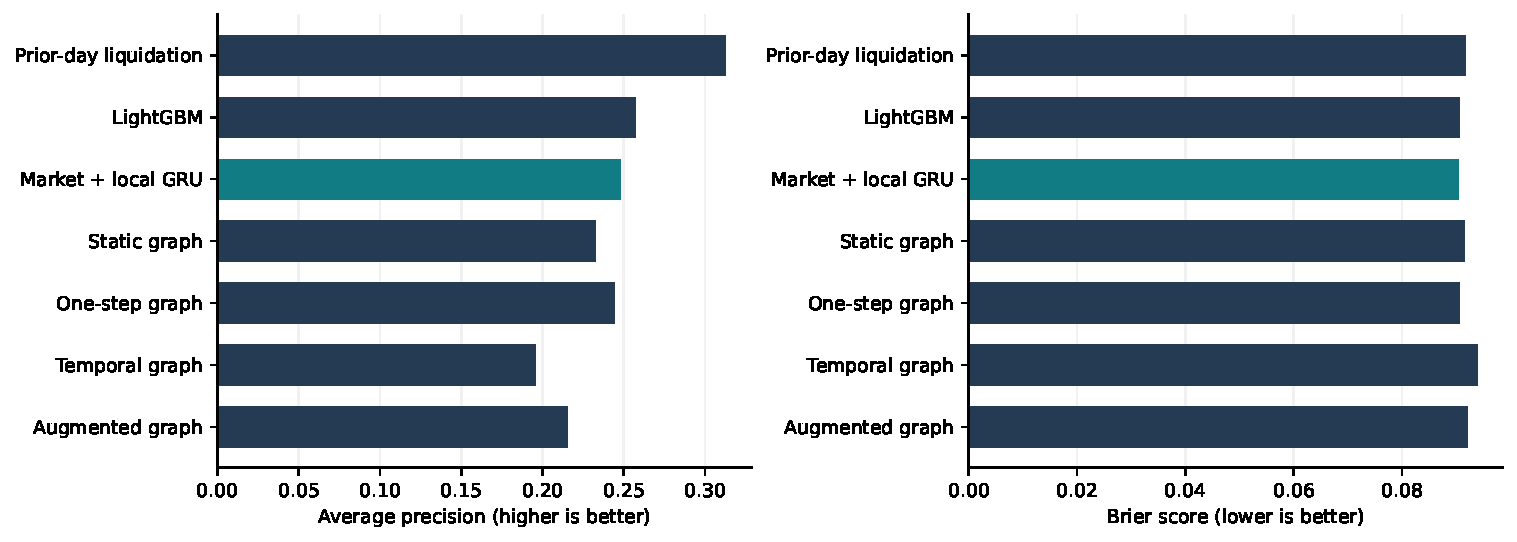
\includegraphics[width=1\textwidth,height=0.33\textheight,keepaspectratio]{../revision/figures/primary_performance.pdf}
\caption{Recomputed clean primary scores from one supplied forecast
ledger. Both horizontal scales begin at zero.}
\end{figure}

Static and one-step graph variants rank ahead of the full temporal graph
in the pooled sample. Adding graph summaries to LightGBM lowers its AP
point estimate. These observations constrain claims about the selected
representation but do not distinguish uninformative links from redundant
inputs, small sample size, weak peer attributes or scope mismatch. They
do not answer the comparison with borrower Health Factor, which remains
unavailable.

\subsection{Calibration, masks and analyst
workload}\label{calibration-masks-and-analyst-workload}

The supplied raw and calibrated graph forecasts yield the following
clean-score comparison.

\Needspace{10\baselineskip}
\begin{longtable}[]{@{}llll@{}}
\caption{Calibration uses earlier calibration blocks; it is frozen
during testing.}\tabularnewline
\toprule\noalign{}
Graph probability & AP & Brier & Log loss \\
\midrule\noalign{}
\endfirsthead
\toprule\noalign{}
Graph probability & AP & Brier & Log loss \\
\midrule\noalign{}
\endhead
\bottomrule\noalign{}
\endlastfoot
Raw ensemble & 0.1930 & 0.0962 & 0.3626 \\
Platt calibrated & 0.1954 & 0.0939 & 0.3319 \\
Isotonic & 0.1617 & 0.0952 & 0.3562 \\
\end{longtable}

\begin{figure}[H]
\centering
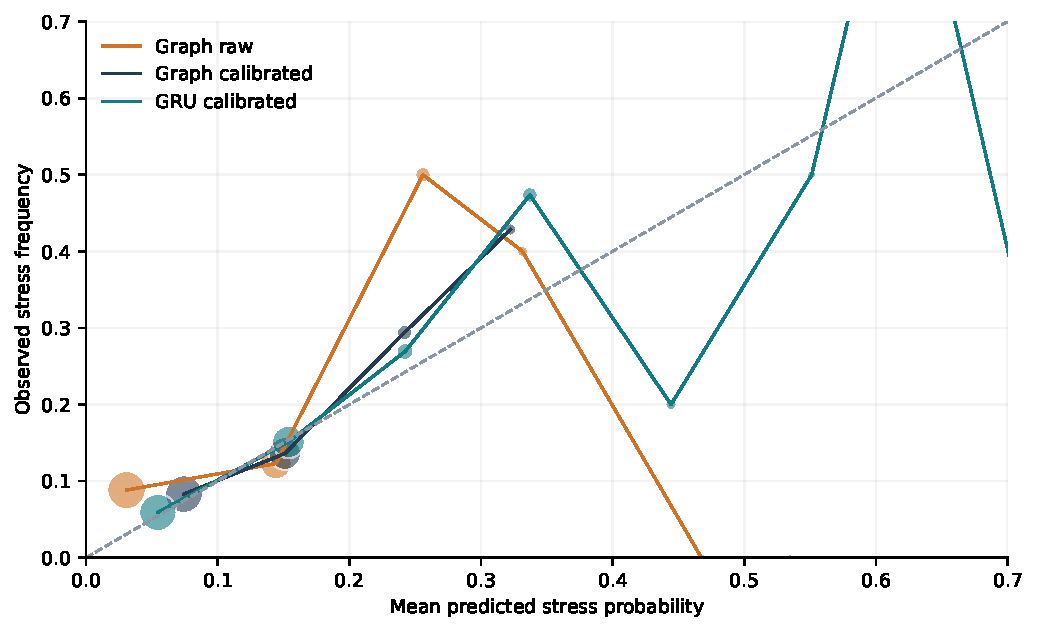
\includegraphics[width=0.78\textwidth,height=0.33\textheight,keepaspectratio]{../revision/figures/calibration_recomputed.pdf}
\caption{Equal-width reliability bins from the same clean ledger. Marker
area reflects occupancy; sparse upper bins remain uncertain.}
\end{figure}

Mean AP changes under thinning are slightly positive at each rate, but
some masks worsen ranking. Probability error moves in the opposite
direction: 99 of 100 masks at 50\% thinning worsen Brier loss. A
favourable deterministic mask would therefore give an incomplete account
of robustness.

\Needspace{10\baselineskip}
\begin{longtable}[]{@{}
  >{\raggedright\arraybackslash}p{(\columnwidth - 8\tabcolsep) * \real{0.2000}}
  >{\raggedright\arraybackslash}p{(\columnwidth - 8\tabcolsep) * \real{0.2000}}
  >{\raggedright\arraybackslash}p{(\columnwidth - 8\tabcolsep) * \real{0.2000}}
  >{\raggedright\arraybackslash}p{(\columnwidth - 8\tabcolsep) * \real{0.2000}}
  >{\raggedright\arraybackslash}p{(\columnwidth - 8\tabcolsep) * \real{0.2000}}@{}}
\caption{100 mask draws per rate. All changes are paired with the same
fitted clean graph.}\tabularnewline
\toprule\noalign{}
\begin{minipage}[b]{\linewidth}\raggedright
Removal
\end{minipage} & \begin{minipage}[b]{\linewidth}\raggedright
Mean AP change
\end{minipage} & \begin{minipage}[b]{\linewidth}\raggedright
AP worse / 100
\end{minipage} & \begin{minipage}[b]{\linewidth}\raggedright
Mean Brier change
\end{minipage} & \begin{minipage}[b]{\linewidth}\raggedright
Brier worse / 100
\end{minipage} \\
\midrule\noalign{}
\endfirsthead
\toprule\noalign{}
\begin{minipage}[b]{\linewidth}\raggedright
Removal
\end{minipage} & \begin{minipage}[b]{\linewidth}\raggedright
Mean AP change
\end{minipage} & \begin{minipage}[b]{\linewidth}\raggedright
AP worse / 100
\end{minipage} & \begin{minipage}[b]{\linewidth}\raggedright
Mean Brier change
\end{minipage} & \begin{minipage}[b]{\linewidth}\raggedright
Brier worse / 100
\end{minipage} \\
\midrule\noalign{}
\endhead
\bottomrule\noalign{}
\endlastfoot
10\% & +0.00216 & 27 & +0.000026 & 58 \\
30\% & +0.00424 & 24 & +0.000157 & 87 \\
50\% & +0.00346 & 36 & +0.000343 & 99 \\
\end{longtable}

\begin{figure}[H]
\centering
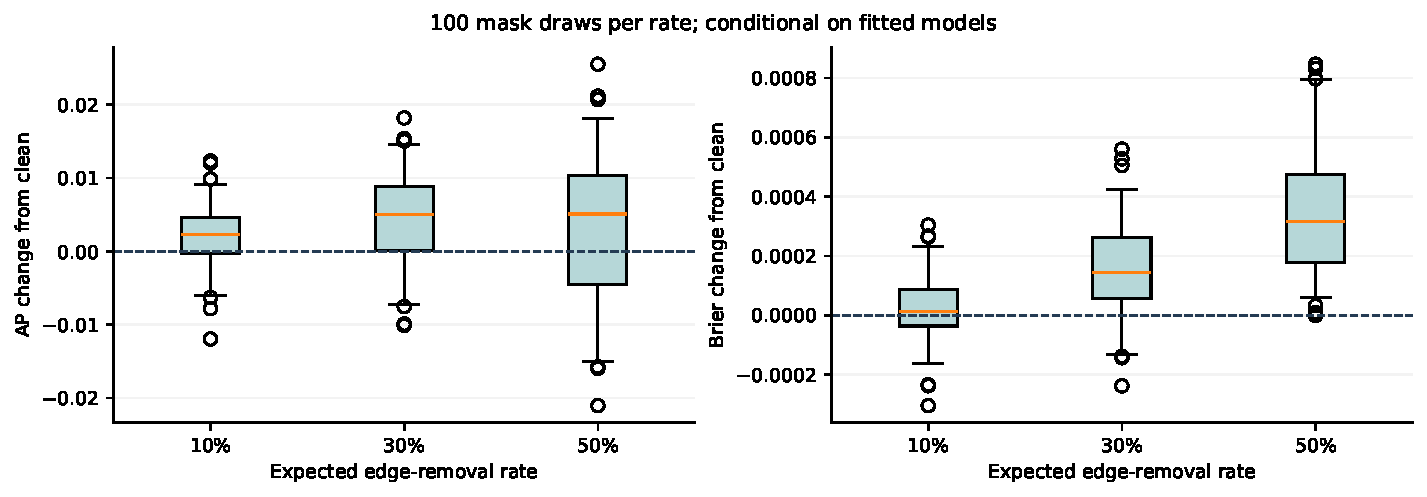
\includegraphics[width=1\textwidth,height=0.33\textheight,keepaspectratio]{../revision/figures/mask_sensitivity.pdf}
\caption{Mask variation conditional on fitted ensembles. Whiskers span
empirical 2.5th-97.5th percentiles, not confidence intervals for future
markets.}
\end{figure}

Original delayed-input scenarios and alternative horizons remain in the
replication tables. They are covariate interventions on observed
outcomes. Review additionally trades fewer automated false warnings
against fewer automated onset detections and a large manual queue.
Without an analyst experiment, reviewed cases cannot be counted as
recovered events.

\Needspace{10\baselineskip}
\begin{longtable}[]{@{}lllll@{}}
\caption{Operational counts from the same supplied primary ledger.
Reviews are not successful detections.}\tabularnewline
\toprule\noalign{}
Rule & Automated alerts & False alerts & Onsets hit & Reviews \\
\midrule\noalign{}
\endfirsthead
\toprule\noalign{}
Rule & Automated alerts & False alerts & Onsets hit & Reviews \\
\midrule\noalign{}
\endhead
\bottomrule\noalign{}
\endlastfoot
Graph & 188 & 151 & 16/70 & 0 \\
Graph + review & 36 & 25 & 6/70 & 241 \\
GRU & 184 & 138 & 20/70 & 0 \\
\end{longtable}

\subsection{Fusion on C and a later chronological
test}\label{fusion-on-c-and-a-later-chronological-test}

The existing gate and nested selection have little ranking separation
from the GRU on C. As fusion was developed after seeing the original
benchmark, these C results support exploratory estimation only.

\Needspace{10\baselineskip}
\begin{longtable}[]{@{}llll@{}}
\caption{Exploratory original C results, 472 forecasts and 53
positives.}\tabularnewline
\toprule\noalign{}
C-only predictor & AP & Brier & Log loss \\
\midrule\noalign{}
\endfirsthead
\toprule\noalign{}
C-only predictor & AP & Brier & Log loss \\
\midrule\noalign{}
\endhead
\bottomrule\noalign{}
\endlastfoot
Graph & 0.1975 & 0.099751 & 0.351594 \\
GRU & 0.3115 & 0.092422 & 0.312513 \\
Fixed half & 0.3059 & 0.093687 & 0.321133 \\
Disagreement heuristic & 0.3096 & 0.093002 & 0.317223 \\
Original gate (penalty 10) & 0.3112 & 0.092402 & 0.313454 \\
Nested selected gate & 0.3113 & 0.092263 & 0.313368 \\
\end{longtable}

The later test has 744 cases/40 positives (5.38\%). Its training q95
thresholds are USD 691,427 for V2 and USD 2,716,455 for V3. These differ
from original C, so prevalence changes are not statements about an
unchanged physical stress boundary.

\Needspace{10\baselineskip}
\begin{longtable}[]{@{}llll@{}}
\caption{Previously unscored later calendar, 744 forecasts and 40
positives; no independent-source claim.}\tabularnewline
\toprule\noalign{}
Later predictor & AP & Brier & Log loss \\
\midrule\noalign{}
\endfirsthead
\toprule\noalign{}
Later predictor & AP & Brier & Log loss \\
\midrule\noalign{}
\endhead
\bottomrule\noalign{}
\endlastfoot
Graph & 0.307427 & 0.048868 & 0.191485 \\
GRU & 0.324161 & 0.046263 & 0.171444 \\
Fixed half & 0.330924 & 0.047430 & 0.179051 \\
Disagreement heuristic & 0.324353 & 0.046305 & 0.171762 \\
Learned gate & 0.322987 & 0.046439 & 0.172463 \\
Expiry + heuristic & 0.324193 & 0.046262 & 0.171428 \\
\end{longtable}

\Needspace{10\baselineskip}
\begin{longtable}[]{@{}
  >{\raggedright\arraybackslash}p{(\columnwidth - 4\tabcolsep) * \real{0.3333}}
  >{\raggedright\arraybackslash}p{(\columnwidth - 4\tabcolsep) * \real{0.3333}}
  >{\raggedright\arraybackslash}p{(\columnwidth - 4\tabcolsep) * \real{0.3333}}@{}}
\caption{Paired 14-day intervals conditional on the later fitted
forecasts. Small magnitudes are retained.}\tabularnewline
\toprule\noalign{}
\begin{minipage}[b]{\linewidth}\raggedright
Minus GRU
\end{minipage} & \begin{minipage}[b]{\linewidth}\raggedright
AP difference {[}95\%{]}
\end{minipage} & \begin{minipage}[b]{\linewidth}\raggedright
Brier difference {[}95\%{]}
\end{minipage} \\
\midrule\noalign{}
\endfirsthead
\toprule\noalign{}
\begin{minipage}[b]{\linewidth}\raggedright
Minus GRU
\end{minipage} & \begin{minipage}[b]{\linewidth}\raggedright
AP difference {[}95\%{]}
\end{minipage} & \begin{minipage}[b]{\linewidth}\raggedright
Brier difference {[}95\%{]}
\end{minipage} \\
\midrule\noalign{}
\endhead
\bottomrule\noalign{}
\endlastfoot
Graph & -0.0167 {[}-0.0752, 0.0754{]} & 0.002605 {[}0.000900,
0.004972{]} \\
Fixed half & 0.0068 {[}-0.0170, 0.0660{]} & 0.001167 {[}0.000334,
0.002317{]} \\
Disagreement heuristic & 0.0002 {[}-0.0030, 0.0038{]} & 0.000042
{[}0.000005, 0.000086{]} \\
Learned gate & -0.0012 {[}-0.0155, 0.0088{]} & 0.000177 {[}0.000030,
0.000377{]} \\
Expiry + heuristic & 0.0000 {[}-0.0001, 0.0007{]} & -0.000001
{[}-0.000010, 0.000000{]} \\
\end{longtable}

The later learned gate has AP 0.3230 versus GRU 0.3242, with a positive
Brier difference. A 50/50 mixture improves the AP point estimate but
worsens Brier/log loss; its AP interval spans zero. Marginal ranking
movement does not establish better probability quality. The
freshness-capped heuristic is almost identical to the GRU because it
ignores the graph for most of this stale-feed regime. Near-equality is
evidence of fallback behaviour, not a new source of predictive
information.

\begin{figure}[H]
\centering
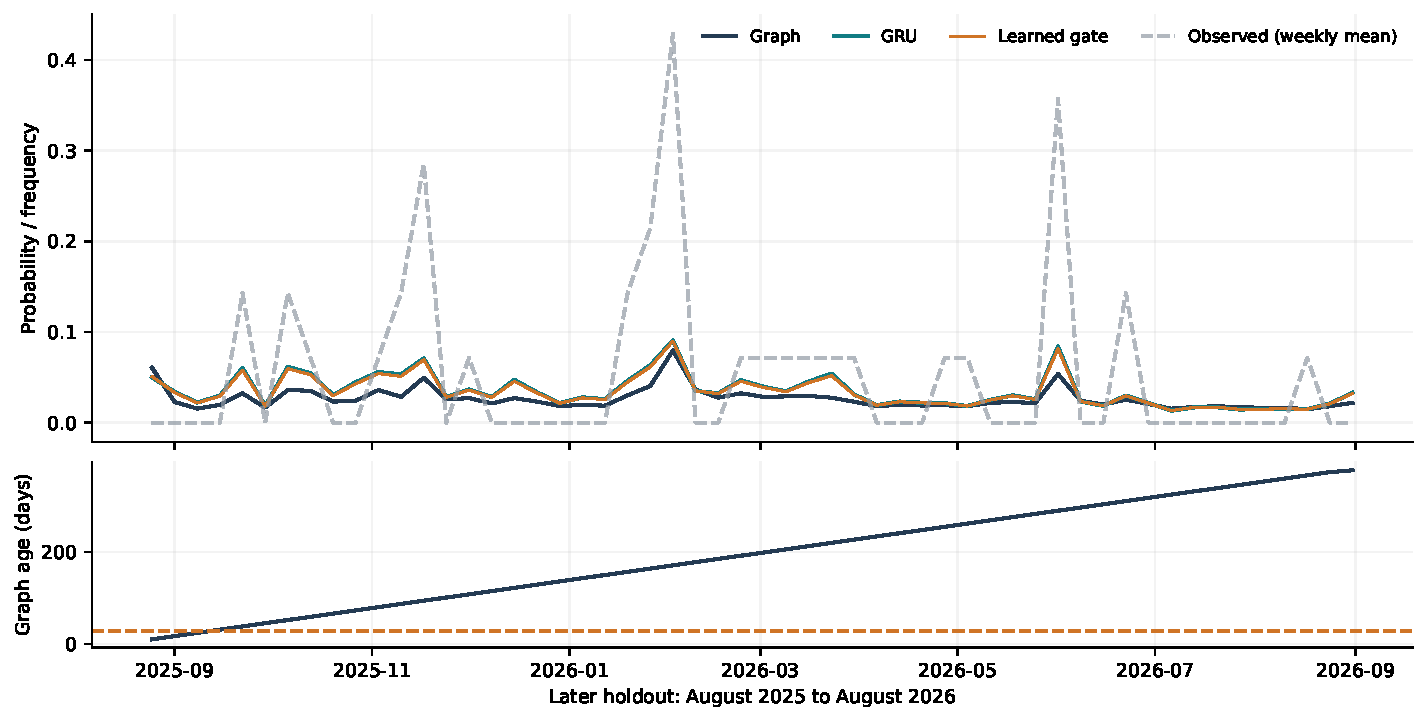
\includegraphics[width=1\textwidth,height=0.33\textheight,keepaspectratio]{../revision/figures/later_holdout_history.pdf}
\caption{Later forecasts and measured graph age. Weekly means aid
display only; scores use unsmoothed daily version-level predictions.}
\end{figure}

\begin{figure}[H]
\centering
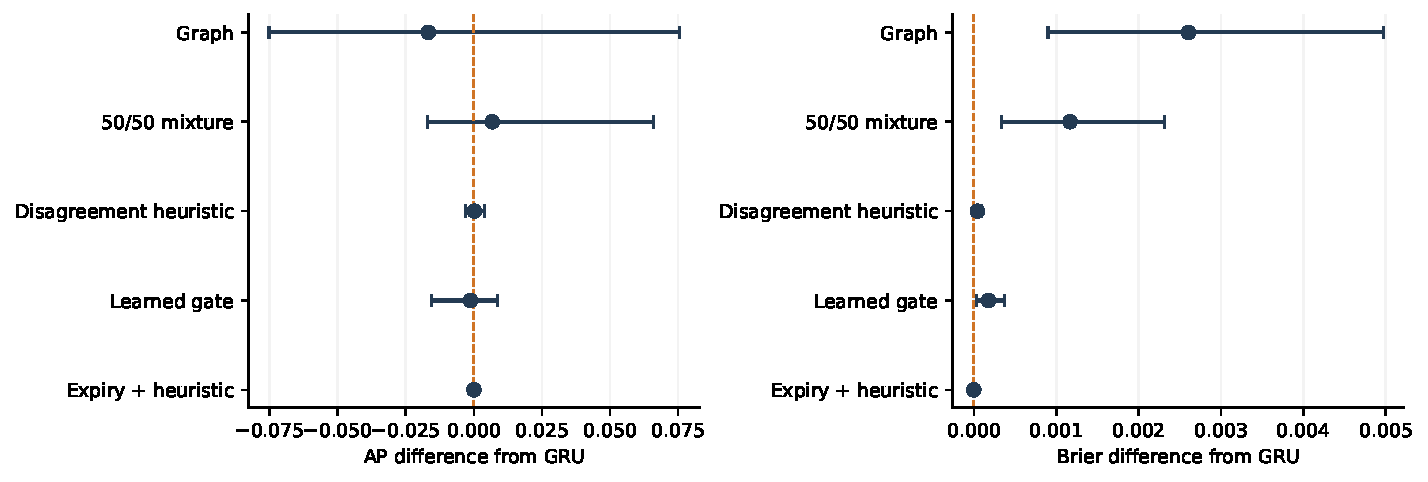
\includegraphics[width=1\textwidth,height=0.33\textheight,keepaspectratio]{../revision/figures/later_holdout_differences.pdf}
\caption{Later paired differences from GRU, using 2,000 14-day
moving-block draws with both versions clustered by date.}
\end{figure}

The experiment tests a frozen gate with renewed expert fits and a
changing age distribution. It cannot isolate age causally from evolving
market regimes. It nevertheless directly challenges the idea that
disagreement alone makes fusion robust to obsolete network observations.
Source freshness is independently observable and should accompany a
learned uncertainty measure.

\subsection{Conditional Compound
transfer}\label{conditional-compound-transfer}

Frozen-source predictions were actually generated. Both Compound
versions have 196 valid test days, with 12 V2/19 V3 positives. Ranking
transfer is weak, especially for the graph. On V3 both source models
rank below target-supervised references, while probability-loss
differences are smaller. On V2 a source model can have lower Brier error
despite weaker ranking, illustrating separate effects of base-rate
alignment and ordering.

\Needspace{10\baselineskip}
\begin{longtable}[]{@{}
  >{\raggedright\arraybackslash}p{(\columnwidth - 8\tabcolsep) * \real{0.2000}}
  >{\raggedright\arraybackslash}p{(\columnwidth - 8\tabcolsep) * \real{0.2000}}
  >{\raggedright\arraybackslash}p{(\columnwidth - 8\tabcolsep) * \real{0.2000}}
  >{\raggedright\arraybackslash}p{(\columnwidth - 8\tabcolsep) * \real{0.2000}}
  >{\raggedright\arraybackslash}p{(\columnwidth - 8\tabcolsep) * \real{0.2000}}@{}}
\caption{Conditional publisher-cohort transfer, 196 days per version.
Target-history q95 scaling is declared.}\tabularnewline
\toprule\noalign{}
\begin{minipage}[b]{\linewidth}\raggedright
Target / model
\end{minipage} & \begin{minipage}[b]{\linewidth}\raggedright
Frozen-source AP
\end{minipage} & \begin{minipage}[b]{\linewidth}\raggedright
Target-fit AP
\end{minipage} & \begin{minipage}[b]{\linewidth}\raggedright
Source Brier
\end{minipage} & \begin{minipage}[b]{\linewidth}\raggedright
Target Brier
\end{minipage} \\
\midrule\noalign{}
\endfirsthead
\toprule\noalign{}
\begin{minipage}[b]{\linewidth}\raggedright
Target / model
\end{minipage} & \begin{minipage}[b]{\linewidth}\raggedright
Frozen-source AP
\end{minipage} & \begin{minipage}[b]{\linewidth}\raggedright
Target-fit AP
\end{minipage} & \begin{minipage}[b]{\linewidth}\raggedright
Source Brier
\end{minipage} & \begin{minipage}[b]{\linewidth}\raggedright
Target Brier
\end{minipage} \\
\midrule\noalign{}
\endhead
\bottomrule\noalign{}
\endlastfoot
V2 GRU & 0.0677 & 0.1500 & 0.0639 & 0.0689 \\
V2 Graph & 0.0604 & 0.1063 & 0.0711 & 0.0937 \\
V3 GRU & 0.1109 & 0.1982 & 0.0899 & 0.0885 \\
V3 Graph & 0.0921 & 0.1972 & 0.0940 & 0.0929 \\
\end{longtable}

\begin{figure}[H]
\centering
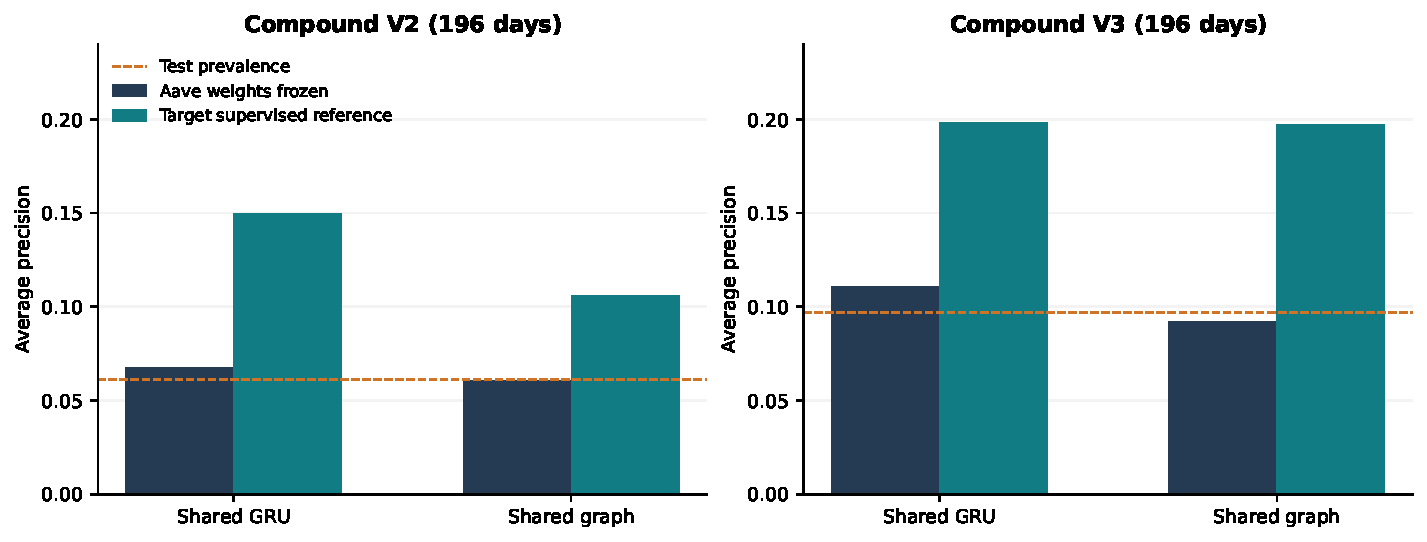
\includegraphics[width=1\textwidth,height=0.33\textheight,keepaspectratio]{../revision/figures/transfer_performance.pdf}
\caption{Executed transfer scores. Dashed lines give target test
prevalence as an uninformative-ranking reference. Missing crisis
neighbourhoods are excluded.}
\end{figure}

On V3, source-minus-target AP differences are -0.0873 for GRU and
-0.1051 for graph, with conditional intervals {[}-0.1758, -0.0239{]} and
{[}-0.1929, -0.0316{]}. These exploratory results show that transfer was
executed and failed to match supervised ranking in the filtered cohort.
They do not establish chain-validated external performance, a
crisis-inclusive benchmark or coverage of every Compound deployment.

\section{Historical account health and independent
validation}\label{historical-account-health-and-independent-validation}

\subsection{Health Factor remains a missing
benchmark}\label{health-factor-remains-a-missing-benchmark}

For a basic position, the conceptual Health Factor is
\[\mathrm{HF}_{u,t}=\frac{\sum_a C_{u,a,t}P_{a,t}\mathrm{LT}_{a,t}}{\sum_a D_{u,a,t}P_{a,t}}.\]
Contract values additionally depend on units, integer rounding,
eligibility and historical implementation rules. Official Aave
interfaces expose account data, and its logic includes version/eMode
behaviour (Aave 2026, 2025). Reserve utilisation and governance
thresholds are not account HF. Liquidated-account samples are not
representative borrower cross-sections.

The supplied Cred sample has 75 observations from January 2021-June 2022
and zero overlap with the primary interval (Cred Protocol n.d.). Its
aggregate collateral/debt arithmetic reproduces supplied HF values,
which is an algebraic identity within one dataset, not chain-state
validation or a contemporary risk panel.

Delivered reconstruction code reads token balances, prices, collateral
flags and configuration at an exact block, applies supported basic
legacy integer rules and compares against \texttt{getUserAccountData}.
Debt-free HF is undefined; unsupported eMode/ABI cases fail explicitly.
Ten training-era account/block requests are included for mechanics
checks. No real historical HF output was generated because archive calls
were denied. Software tests are not represented as empirical validation.

\subsection{The required incremental-information
comparison}\label{the-required-incremental-information-comparison}

A suitable panel must enumerate borrowers as known at each origin, not
select future liquidation recipients. At a block strictly before
midnight it should measure debt-weighted HF shares, buffer distributions
and coverage. For example,
\[S_t(\tau)=\frac{\sum_u D_{u,t}\mathbb{1}\{\mathrm{HF}_{u,t}<\tau\}}{\sum_u D_{u,t}}\]
requires a documented borrower denominator. The next comparison must
hold cohort, target, dates and calibration fixed across local/market,
local/market/HF and local/market/HF/graph models. This ablation has not
run. Current findings concern network value relative to the available
local inputs, not the best obtainable loan-health information.

\subsection{Compound semantics and
access}\label{compound-semantics-and-access}

Compound V2 emits \texttt{LiquidateBorrow}; Compound III uses absorption
and later collateral-sale mechanics (Compound 2026b, 2026a). Its
\texttt{AbsorbDebt} event contains \texttt{basePaidOut} and
\texttt{usdValue} (Compound Finance 2026). We retain the emitted
valuation without automatically renaming it borrower principal or seized
collateral. Reconciliation must specify which quantity a published daily
column measures, deployment coverage and UTC boundaries. V2 repayment
and seized collateral also need separate historical valuation paths.

Network identity and a historical block header were obtainable.
Historical state/log requests returned HTTP 403 on the tested routes,
and no authenticated archive endpoint was configured. Access reports
distinguish failure from an empty history. The supplied read-only
collector checks continuous block coverage, event uniqueness,
removed-log flags and block hashes and can compare a second endpoint. It
covers a specified Ethereum Compound III USDC deployment, not complete
V2/V3 reconciliation, and has no claimed executed validation result.

\section{Discussion}\label{discussion}

\subsection{Interpreting the negative
evidence}\label{interpreting-the-negative-evidence}

The original and later tests constrain a practical claim: this network
representation and disagreement gate do not establish a stable advantage
over timely local/market forecasting. The evidence includes exact score
recomputation, a full primary refit, multiple corruption masks and a
previously unscored calendar. It is weaker than a universal assertion
that financial networks are uninformative. Only two source-labelled Aave
series, one graph construction and a small family of encoders are
tested.

Local liquidation history may already encode pressure associated with
exposure links. Weekly global measurements may be too coarse for
next-day account events. Peer attributes describe scale/exposure rather
than independently labelled distress. Additional complexity competes
with few independent stress episodes. Global graph coverage and Ethereum
outcomes are imperfectly aligned. The present design cannot identify the
relative contribution of these explanations, and absent HF controls
prevent a stronger conditional-information claim.

Thinning separates sensitivity from economic information. Removing links
can attenuate unhelpful messages and improve some ranks while worsening
probability magnitude. This does not mean data loss is intrinsically
protective. It argues for reporting distributions across specified masks
and calibration diagnostics under the same frozen forecast rule.

\subsection{Reliability needs source
metadata}\label{reliability-needs-source-metadata}

Ensemble disagreement is not a certificate of input validity. Members
can agree on stale or mismeasured data. The later window deliberately
exposes this problem. Its expiry comparator mostly reproduces local
forecasts: a conservative behaviour, not a demonstrated network gain.
Monitoring should display age, coverage and supported-regime flags
alongside probabilities. Governance policies also need intervention
costs and financial consequences, which forecast scores alone cannot
establish.

The companion local-currency adaptive-governance repository concerns
policy responses to delayed observations. It is a separate modelling
project, not independent empirical evidence for these forecasts. Neither
predictive differences nor directed aggregate exposures alone justify an
assertion of causal contagion or a welfare-improving parameter
intervention.

\subsection{Selection and measurement}\label{selection-and-measurement}

Transfer is a real procedure with saved weights, but deleting a crisis
day is particularly damaging to a tail estimand. The 196-day cohort is
explicit about eligibility yet remains selected by publisher filtering.
It must not be advertised as a fully validated cross-protocol warning
system. Matching published Aave series can establish compatibility while
leaving common upstream dependencies unresolved. Independent
verification requires event identities and a declared valuation map, not
high correlation alone.

HF reconstruction has an analogous boundary: an equation is insufficient
when balances accrue interest, collateral eligibility changes and
protocol implementations evolve. Unsupported components must remain
missing rather than become reassuring zeros. Selected-account checks can
validate mechanics but cannot supply a representative risk distribution
without an enumerated borrower universe.

\subsection{Statistical and submission
limits}\label{statistical-and-submission-limits}

Effective information is closer to independent stress episodes than
total version-days. Moving blocks preserve local clustering but cannot
guarantee coverage under future regimes. The later window has only 40
positives and an increasingly obsolete graph. AP depends on prevalence;
thresholds differ across cohorts. All source-quality decisions and model
fits are retained, but no independent preregistration is claimed.

Independent Compound reconciliation and a representative validated HF
comparison remain material evidence gaps. A claim of network value
beyond loan health cannot be made without the latter. This is a revised
research manuscript for scientific review, with completed and blocked
tasks separated below. Journal quartile and acceptance are not inferred
from architecture complexity or document formatting.

\section{Conclusion}\label{conclusion}

The selected temporal graph and reliability gate do not demonstrate
stable improvement over local/market alternatives across the original
Aave study and a later chronological window. Prior liquidation is a
strong ranking comparator; calibration affects probability error;
missing-link ranking changes can diverge from probability quality.
Executed source-weight transfer is weak and conditional on important
calendar/measurement assumptions. The package preserves negative
results, distinct runs and unfinished validation. Additional network
value relative to historical borrower health remains an empirical
question.

\section{Reproducibility and evidence
status}\label{reproducibility-and-evidence-status}

\Needspace{10\baselineskip}
\begin{longtable}[]{@{}
  >{\raggedright\arraybackslash}p{(\columnwidth - 4\tabcolsep) * \real{0.3333}}
  >{\raggedright\arraybackslash}p{(\columnwidth - 4\tabcolsep) * \real{0.3333}}
  >{\raggedright\arraybackslash}p{(\columnwidth - 4\tabcolsep) * \real{0.3333}}@{}}
\caption{Completed analyses and unresolved scientific requirements at
this revision.}\tabularnewline
\toprule\noalign{}
\begin{minipage}[b]{\linewidth}\raggedright
Analysis
\end{minipage} & \begin{minipage}[b]{\linewidth}\raggedright
Status
\end{minipage} & \begin{minipage}[b]{\linewidth}\raggedright
Interpretive boundary
\end{minipage} \\
\midrule\noalign{}
\endfirsthead
\toprule\noalign{}
\begin{minipage}[b]{\linewidth}\raggedright
Analysis
\end{minipage} & \begin{minipage}[b]{\linewidth}\raggedright
Status
\end{minipage} & \begin{minipage}[b]{\linewidth}\raggedright
Interpretive boundary
\end{minipage} \\
\midrule\noalign{}
\endhead
\bottomrule\noalign{}
\endlastfoot
Original metric audit & Executed & 47 rows recomputed; no independent
chain claim \\
Primary model refit & Executed & Software-sensitive outputs kept
separate \\
100-mask analysis & Executed & Conditional on fitted ensembles \\
Later fusion test & Executed & New calendar, same source, stale graph \\
Aave-to-Compound transfer & Executed conditionally & Filtered daily
source; UTC/valuation assumptions \\
Compound raw-log reconciliation & Blocked & Historical log access
denied \\
Representative historical HF & Not completed & Selected old sample is
insufficient \\
Network beyond HF comparison & Not executed & Requires validated
borrower-health panel \\
\end{longtable}

The package contains forecast ledgers, original sensitivity outputs,
source hashes, transfer/later-window weights, scaling/calibration
metadata, specifications, code and tests. Large upstream archives are
downloaded from cited sources; small derived panels/graphs accompany the
review package. Credentials are read from environment variables and
excluded from the repository. Original and refitted primary ledgers stay
separate. Tables are generated directly from score files.

The authors must confirm final authorship, affiliations,
funding/competing-interest statements and the selected journal's
disclosure requirements before submission. No external journal
submission is performed by this revision.

\newpage

\section{References}\label{references}

\section*{References}\label{bibliography}
\addcontentsline{toc}{section}{References}

\phantomsection\label{refs}
\begin{CSLReferences}{1}{0}
\bibitem[\citeproctext]{ref-aavelogic}
Aave. 2025. {`Aave V3 Core: GenericLogic.sol'}.
\url{https://github.com/aave/aave-v3-core/blob/master/contracts/protocol/libraries/logic/GenericLogic.sol}.

\bibitem[\citeproctext]{ref-aavepool}
---------. 2026. {`Aave V3 Pool Contract: getUserAccountData'}.
\url{https://aave.com/docs/aave-v3/smart-contracts/pool}.

\bibitem[\citeproctext]{ref-chaffard2026}
Chaffard, Owen. 2026. {`Stablecoin {DeFi} Hourly Dataset, 2026-11-15'}.
Zenodo, version v192. \url{https://doi.org/10.5281/zenodo.24245638}.

\bibitem[\citeproctext]{ref-chiu2026}
Chiu, Jonathan, and Furkan Danisman. 2026. {`{DeFi} Lending: Returns,
Leverage, and Liquidation Risk'}. Staff Analytical Paper 2026-13. Bank
of Canada. \url{https://doi.org/10.34989/sap-2026-13}.

\bibitem[\citeproctext]{ref-cho2014}
Cho, Kyunghyun, Bart van Merriënboer, Caglar Gulcehre, Dzmitry Bahdanau,
Fethi Bougares, Holger Schwenk, and Yoshua Bengio. 2014. {`Learning
Phrase Representations Using {RNN} Encoder--Decoder for Statistical
Machine Translation'}. In \emph{Proceedings of the 2014 Conference on
Empirical Methods in Natural Language Processing}, 1724--34.
\url{https://doi.org/10.3115/v1/D14-1179}.

\bibitem[\citeproctext]{ref-compoundv3}
Compound. 2026a. {`Compound III Documentation: Liquidation'}.
\url{https://docs.compound.finance/liquidation/}.

\bibitem[\citeproctext]{ref-compoundv2}
---------. 2026b. {`Compound V2 Documentation: cTokens and Liquidation
Events'}. \url{https://docs.compound.finance/v2/ctokens/}.

\bibitem[\citeproctext]{ref-cometcode}
Compound Finance. 2026. {`Comet: Main Interface, Absorption Logic and
Ethereum USDC Deployment'}.
\url{https://github.com/compound-finance/comet/tree/f766f51583c23acc33b2a7824654ef2029a96804}.

\bibitem[\citeproctext]{ref-credhf}
Cred Protocol. n.d. {`Aave V2 Health Factor Dataset'}. Accessed 17
November 2026.
\url{https://github.com/credprotocol/Aave-V2-Health-Factor-Dataset}.

\bibitem[\citeproctext]{ref-geifman2017}
Geifman, Yonatan, and Ran El-Yaniv. 2017. {`Selective Classification for
Deep Neural Networks'}. In \emph{Advances in Neural Information
Processing Systems}. Vol. 30.
\url{https://proceedings.neurips.cc/paper_files/paper/2017/hash/4a8423d5e91fda00bb7e46540e2b0cf1-Abstract.html}.

\bibitem[\citeproctext]{ref-gneiting2007}
Gneiting, Tilmann, and Adrian E. Raftery. 2007. {`Strictly Proper
Scoring Rules, Prediction, and Estimation'}. \emph{Journal of the
American Statistical Association} 102 (477): 359--78.
\url{https://doi.org/10.1198/016214506000001437}.

\bibitem[\citeproctext]{ref-guo2017}
Guo, Chuan, Geoff Pleiss, Yu Sun, and Kilian Q. Weinberger. 2017. {`On
Calibration of Modern Neural Networks'}. In \emph{Proceedings of the
34th International Conference on Machine Learning}, 70:1321--30. PMLR.
\url{https://proceedings.mlr.press/v70/guo17a.html}.

\bibitem[\citeproctext]{ref-hamilton2017}
Hamilton, William L., Rex Ying, and Jure Leskovec. 2017. {`Inductive
Representation Learning on Large Graphs'}. In \emph{Advances in Neural
Information Processing Systems}. Vol. 30.
\url{https://arxiv.org/abs/1706.02216}.

\bibitem[\citeproctext]{ref-iftikhar2025}
Iftikhar, Erum, Wei Wei, and John Cartlidge. 2025. {`Automated Risk
Management Mechanisms in {DeFi} Lending Protocols: A Crosschain
Comparative Analysis of Aave and Compound'}. arXiv preprint 2506.12855.
\url{https://doi.org/10.48550/arXiv.2506.12855}.

\bibitem[\citeproctext]{ref-ke2017}
Ke, Guolin, Qi Meng, Thomas Finley, Taifeng Wang, Wei Chen, Weidong Ma,
Qiwei Ye, and Tie-Yan Liu. 2017. {`{LightGBM}: A Highly Efficient
Gradient Boosting Decision Tree'}. In \emph{Advances in Neural
Information Processing Systems}. Vol. 30.
\url{https://proceedings.neurips.cc/paper_files/paper/2017/hash/6449f44a102fde848669bdd9eb6b76fa-Abstract.html}.

\bibitem[\citeproctext]{ref-kunsch1989}
Künsch, Hans R. 1989. {`The Jackknife and the Bootstrap for General
Stationary Observations'}. \emph{The Annals of Statistics} 17 (3):
1217--41. \url{https://doi.org/10.1214/aos/1176347265}.

\bibitem[\citeproctext]{ref-lakshminarayanan2017}
Lakshminarayanan, Balaji, Alexander Pritzel, and Charles Blundell. 2017.
{`Simple and Scalable Predictive Uncertainty Estimation Using Deep
Ensembles'}. In \emph{Advances in Neural Information Processing
Systems}. Vol. 30.
\url{https://proceedings.neurips.cc/paper/2017/hash/9ef2ed4b7fd2c810847ffa5fa85bce38-Abstract.html}.

\bibitem[\citeproctext]{ref-lehar2022}
Lehar, Alfred, and Christine A. Parlour. 2022. {`Systemic Fragility in
Decentralised Markets'}. BIS Working Papers 1062. Bank for International
Settlements.
\url{https://www.bis.org/publications/working-paper-1062-systemic-fragility-decentralised-markets}.

\bibitem[\citeproctext]{ref-ovadia2019}
Ovadia, Yaniv, Emily Fertig, Jie Ren, Zachary Nado, D. Sculley,
Sebastian Nowozin, Joshua V. Dillon, Balaji Lakshminarayanan, and Jasper
Snoek. 2019. {`Can You Trust Your Model's Uncertainty? Evaluating
Predictive Uncertainty Under Dataset Shift'}. In \emph{Advances in
Neural Information Processing Systems}. Vol. 32.
\url{https://proceedings.neurips.cc/paper/2019/hash/8558cb408c1d76621371888657d2eb1d-Abstract.html}.

\bibitem[\citeproctext]{ref-qin2021}
Qin, Kaihua, Liyi Zhou, Pablo Gamito, Philipp Jovanovic, and Arthur
Gervais. 2021. {`An Empirical Study of {DeFi} Liquidations: Incentives,
Risks, and Instabilities'}. In \emph{Proceedings of the 21st ACM
Internet Measurement Conference}, 336--50.
\url{https://doi.org/10.1145/3487552.3487811}.

\bibitem[\citeproctext]{ref-saito2015}
Saito, Takaya, and Marc Rehmsmeier. 2015. {`The Precision-Recall Plot Is
More Informative Than the {ROC} Plot When Evaluating Binary Classifiers
on Imbalanced Datasets'}. \emph{PLOS ONE} 10 (3): e0118432.
\url{https://doi.org/10.1371/journal.pone.0118432}.

\bibitem[\citeproctext]{ref-schuler2026}
Schuler, Katrin. 2026. {`Frictions in {DeFi} Liquidations: Evidence from
the {Aave V2} Main Market'}. SSRN working paper, revised 6 June 2026.
\url{https://ssrn.com/abstract=6522500}.

\bibitem[\citeproctext]{ref-shu2026}
Shu, Aijie, Wenbin Wu, Gbenga Ibikunle, and Fengxiang He. 2026.
{`{DeXposure-FM}: A Time-Series, Graph Foundation Model for Credit
Exposures and Stability on Decentralized Financial Networks'}. arXiv
preprint 2602.03981, version 2.
\url{https://doi.org/10.48550/arXiv.2602.03981}.

\bibitem[\citeproctext]{ref-wu2025}
Wu, Wenbin, Kejiang Qian, Alexis Lui, Christopher Jack, Yue Wu, Peter
McBurney, Fengxiang He, and Bryan Zhang. 2025. {`{DeXposure}: A Dataset
and Benchmarks for Inter-Protocol Credit Exposure in Decentralized
Financial Networks'}. arXiv preprint 2511.22314.
\url{https://doi.org/10.48550/arXiv.2511.22314}.

\end{CSLReferences}

\end{document}